% EHCI QH 队列与 USB 键盘数据通路问答笔记（Tiny210 / xv6）
% 编译：xelatex ehci-qh-notes.tex（两遍，生成目录）
\documentclass[11pt,a4paper]{ctexart}
\usepackage[margin=2.2cm]{geometry}
\usepackage{amsmath}
\usepackage{graphicx}
\usepackage{booktabs}
\usepackage{tabularx}
\usepackage{array}
\usepackage{xcolor}
\usepackage{fancyvrb}
\usepackage{enumitem}
\usepackage[colorlinks=true,linkcolor=blue!50!black,urlcolor=blue!50!black]{hyperref}

\setlist{itemsep=2pt,topsep=4pt}
\setlength{\emergencystretch}{3em}
\sloppy
\DeclareRobustCommand{\code}[1]{\texttt{\detokenize{#1}}}
\DefineVerbatimEnvironment{codeblock}{Verbatim}{frame=single,fontsize=\small,framesep=3mm,rulecolor=\color{gray!60}}
\newenvironment{note}{\par\smallskip\noindent\begin{tabular}{|p{0.95\linewidth}}}{\end{tabular}\par\smallskip}

\title{EHCI QH 队列与 USB 键盘数据通路\\\large Tiny210（S5PV210）xv6 问答笔记}
\author{}
\date{2026 年 11 月 16 日}

\begin{document}
\maketitle

\begin{abstract}
本文整理关于 Tiny210 上 xv6 EHCI 驱动的一组问答：HC 是什么，
\code{head_qh} 与 \code{anchor_qh} 的区别，1024 项帧表与“当前帧”，
键盘中断 QH 如何进入周期调度，\code{usb_submit_urb} 挂的是什么，中断里如何摘下完成的 qTD，
\code{input_register_device} 与 kbd handler 的关系，以及 MT7601U 批量接收队列的处理时机。
文中的地址、口号和 QH 物理地址都取自实板日志：Hub 为地址 1，有线键盘 2a7a:8a47 为地址 2（Hub 口 3），
MT7601U 为地址 3（Hub 口 4）。
\end{abstract}

\tableofcontents
\bigskip

\section{术语}


\begin{description}
  \item[HC] Host Controller，主机控制器。这里指 S5PV210 片上的 EHCI 硬件（寄存器基址 \code{0xEC200000}，IRQ 55）。
    它会自己做 DMA：CPU 在内存里搭好 QH/qTD 链表，把入口地址写进 \code{PERIODICLIST}/\code{ASYNCLIST} 寄存器；
    之后由 HC 自己读链表、在 USB 线上发包、把结果写回 qTD，CPU 不参与每个包。
  \item[QH] Queue Head，每个端点一个。描述“对哪个设备的哪个端点、以什么速度、经哪个 Hub 的 TT 通信”（\code{epchar}/\code{epcap}），
    并用 \code{horiz} 指针把 QH 串成调度链表。
  \item[qTD] Queue Element Transfer Descriptor，一次传输（transfer）。挂在 QH 的 \code{next} 队列下，含 PID、长度、缓冲区页指针和状态 token。
  \item[overlay] QH 内嵌的一份 qTD 工作区。HC 把当前 qTD 复制进来执行，执行完写回 qTD，再沿 \code{qtd->next} 前进。
  \item[dummy qTD] 每个 QH 队尾的一个 Halted、非 Active 的空 qTD。HC 停在它上面就什么也不做；新传输通过“把旧 dummy 改成真 qTD、再接一个新 dummy”的方式挂上（见 \ref{sec:submit} 节）。
  \item[TT] Transaction Translator，高速 Hub 里的事务翻译器。低速/全速设备挂在高速 Hub 下时，HC 发 SSPLIT/CSPLIT 给 TT，由 TT 在低速总线上代发 IN/OUT。
\end{description}

\section{\texorpdfstring{两条调度链表：\code{head_qh} 与 \code{anchor_qh}}{两条调度链表：head qh 与 anchor qh}}

两者在硬件上是同一种 \code{struct qh}，就是 \code{qhs[]} 池里的前两个（\code{qhs[0]}、\code{qhs[1]}）。
名字只是软件里的指针名；HC 是靠“从哪条路走到它”和“字段的值”来区别对待的。

\begin{center}
\begin{tabularx}{\linewidth}{>{\bfseries}l X X}
\toprule
 & \code{head_qh} & \code{anchor_qh} \\
\midrule
谁指向它 & \code{ASYNCLIST} 寄存器 & 帧表 \code{frame_list} 的全部 1024 项 \\
所在调度 & 异步调度（控制、批量） & 周期调度（中断） \\
链表形状 & 环：\code{horiz} 转一圈回到自己 & 单链：\code{horiz} 一直走到 T（结束） \\
关键位 & \code{epchar.H = 1}（回收头） & \code{epcap.S-mask = 0} \\
作用 & HC 转一圈回到 H=1 的 QH，若这一圈没有做任何事就暂停，避免空转 & S-mask 为 0 的周期 QH 在任何微帧都不执行，HC 只沿它的 \code{horiz} 往下走 \\
token & Halted，从不发包 & Halted，从不发包 \\
\bottomrule
\end{tabularx}
\end{center}

两者都不承载传输，只是两条链表的固定入口（“钩子”）。

\begin{codeblock}
ehci_start:
  head_qh   = &qhs[0];  head_qh->horiz = phys(head_qh) | QH;  // 自己指自己，H=1
  anchor_qh = &qhs[1];  anchor_qh->horiz = T;                 // S-mask 0
  for(i = 0; i < 1024; i++)
    frame_list[i] = phys(anchor_qh) | LINK_QH;                // Typ = 01 (QH)
  wr(PERIODICLIST, phys(frame_list));
  wr(ASYNCLIST,    phys(head_qh));
  wr(USBCMD, ITC(1) | PSE | ASE | RUN);
\end{codeblock}

\section{1024 项帧表与“当前帧”}


\subsection{帧表的作用}

帧表是 EHCI 规定的硬件结构：一个 1024 项的数组（\code{USBCMD} 帧表大小字段为 0 时），每项对应 1 ms，
是“这一毫秒要做哪些周期事务”的链表入口。

\begin{itemize}
  \item \textbf{Linux 的做法}：不同的项指向不同的 QH 组合，用来实现不同的轮询间隔。例如 bInterval = 8 的端点只从 $n = 0, 8, 16, \dots$ 这些项挂进去，所以每 8 ms 才被轮询一次。
  \item \textbf{xv6 的做法}：1024 项全部指向同一个 \code{anchor_qh}，所以挂在 anchor 后面的每个中断端点每 1 ms 都被问一次。键盘描述符里的 bInterval = 10 因此没有生效。
  \item \textbf{为什么要隔一个 anchor}：
    \begin{itemize}
      \item 加一个或删一个中断 QH，只需要改 \code{anchor_qh->horiz} 这一个指针，而不是改写 1024 项；
      \item 没有任何中断端点时链表也不为空：每项指向 anchor，anchor 的 \code{horiz} 为 T，HC 走一下就结束。
    \end{itemize}
\end{itemize}

\subsection{当前帧}

“当前帧”指 HC 此刻正在执行的那 1 毫秒，对应帧表的第 $n$ 项：
\[
  n = \texttt{FRINDEX} \gg 3 \quad (\text{bit } 12{:}3,\ 0 \le n \le 1023)
\]
\begin{itemize}
  \item \code{FRINDEX} 是硬件计数器，HC 运行后每 125\,µs（一个微帧）自动加 1；低 3 位是微帧号 µ0–µ7。
  \item 每 1 ms $n$ 加 1，到 1023 后回到 0，1.024 s 转一圈。
\end{itemize}

每个微帧开始时，HC：
\begin{enumerate}
  \item 读 \code{frame_list[FRINDEX >> 3]}，即当前帧的链表入口；
  \item 沿链表走：\code{anchor_qh} $\rightarrow$ 键盘 QH $\rightarrow \dots \rightarrow$ T；
  \item 对每个 QH 看 S-mask/C-mask 是否命中当前微帧；命中且 overlay 里的 qTD 为 Active 就发包；
  \item 周期调度走完后，本微帧剩余时间去转异步环。
\end{enumerate}

在 xv6 里，因为 1024 项内容相同，无论 $n$ 是几走的都是同一条链表，所以“当前是第几帧”对结果没有影响；
它只在 Linux 那种每项内容不同的帧表里才起作用。

\section{键盘 QH 如何进入周期调度}

\label{sec:enter}

\code{PERIODICLIST} 寄存器里只存帧表的基地址。QH 并不“写进”这个寄存器，而是被链进帧表能走到的链表里，分三步。

\begin{enumerate}
  \item \textbf{开机（\code{ehci_start}）}：帧表 1024 项都写成 \code{phys(anchor_qh) | QH}，然后写 \code{PERIODICLIST} 并打开 \code{USBCMD.PSE}。这时 anchor 的 \code{horiz} 为 T。
  \item \textbf{probe 第一次 \code{usb_submit_urb}}：\code{ehci_submit_urb} 发现 \code{e->intr[1] == 0}，调用
    \code{qh_create_intr(2, 1, LOW, 8, hub=1, port=3)}：
\begin{codeblock}
q->epchar = 2 | 1<<8 | LOW<<12 | 8<<16;          // = 0x00081102，RL=0，DTC=0
q->epcap  = 1<<30 | 0x01 | 0x1c<<8 | 1<<16 | 3<<23; // = 0x41811c01
q->next   = phys(q->dummy);                       // 队列里只有 dummy
q->horiz  = anchor_qh->horiz;                     // = T
dsb();
anchor_qh->horiz = phys(q) | LINK_QH;             // ← 这一次写就挂上了
\end{codeblock}
    最后这一次对齐的 32 位写就是“挂上去”的那一刻，所以不需要先停周期调度。实板日志：
\begin{codeblock}
usb-xfer: qh-intr qh=204d5e20 addr=2 ep=1 speed=1 mps=8 tt=1/3
\end{codeblock}
  \item \textbf{之后每 1 ms}：\code{frame_list[n]} $\rightarrow$ \code{anchor_qh}（不执行）$\rightarrow$ 键盘 QH。
    µ0 命中 S-mask 位 0，发 SSPLIT；µ2–µ4 命中 C-mask \code{0x1c}，发 CSPLIT 取结果。
\end{enumerate}

\begin{center}
\begin{tabular}{l l l}
\toprule
字段 & 值 & 含义 \\
\midrule
epchar.RL & 0 & 周期 QH 必须为 0 \\
epchar.DTC & 0 & 数据翻转位由 HC 记在 overlay 里 \\
epchar.EPS & 01 & 低速 \\
epcap.S-mask & \code{0x01} & µ0 发 SSPLIT \\
epcap.C-mask & \code{0x1c} & µ2、µ3、µ4 发 CSPLIT \\
epcap.Hub / Port & 1 / 3 & split 发给 Hub 1 的口 3 的 TT \\
\bottomrule
\end{tabular}
\end{center}

QH 一旦挂上就一直留在链表里，来来去去的只是 qTD。

\section{\texorpdfstring{\code{usb_submit_urb} 挂的是什么}{usb submit urb 挂的是什么}}
\label{sec:submit}

qTD 挂在\textbf{键盘自己的中断 QH} 上，不挂在 \code{anchor_qh} 上。\code{anchor_qh} 下面从来不挂 qTD。

\begin{codeblock}
frame_list[n] --> anchor_qh --horiz--> 键盘 QH(地址2 EP1) --horiz--> T
                  (S-mask=0，不执行)        |
                                            +--next--> qTD(IN 8B, Active) --> dummy
\end{codeblock}

\begin{itemize}
  \item \textbf{horiz（横向）}：把 QH 串起来，表示“这一帧要访问哪些端点”。anchor 只在这条线上。
  \item \textbf{next（纵向）}：每个 QH 自己的 qTD 队列，表示“这个端点要做哪些传输”。
\end{itemize}

\code{usb_submit_urb} $\rightarrow$ \code{ehci_submit_urb} 做两件事：
\begin{enumerate}
  \item \textbf{只在第一次}：\code{qh_create_intr} 建 QH 并插到 anchor 的 \code{horiz} 后面（第 \ref{sec:enter} 节）。
  \item \textbf{每次}：\code{qtd_fill} 准备一个 IN 8 字节、带 IOC 的 qTD，\code{qh_append(q, t, t)} 用 dummy 法挂到键盘 QH 的 \code{next} 队列末尾，并登记到 \code{intrs[]}。
\end{enumerate}

dummy 法的要点：
\begin{enumerate}
  \item 申请一个新 dummy；
  \item 把新 qTD 的内容（除 token）复制进旧 dummy，旧 dummy 的 \code{next} 指向新 dummy；
  \item 最后才把旧 dummy 的 token 写成 Active。
\end{enumerate}
最后这一次 32 位写就是“发布”：HC 下次访问这个 QH 时发现当前 qTD 变成 Active，就开始执行，永远看不到半成品。

之后每次 rx\_work 处理完报告再 submit，只往键盘 QH 下挂一个新的 qTD，anchor 和 \code{horiz} 链都不再动。

\section{中断里如何摘下完成的 qTD}


中断处理\textbf{不遍历} anchor 的链表，摘的时候也\textbf{不改}硬件链表。

\subsection{\texorpdfstring{查软件登记表 \code{intrs[4]}}{查软件登记表 intrs[4]}}
\begin{itemize}
  \item 每次 \code{ehci_submit_urb} 挂 qTD 时，在 \code{intrs[]} 登记一行 \texttt{\{urb, qh, qtd\}}。
  \item 中断到来，\code{ehci_intr_reap} 只扫这 4 个槽：哪个槽的 \code{qtd->token} 的 Active 位已为 0，就是 HC 做完的。
  \item 这样做的原因：
    \begin{itemize}
      \item 中断只告诉 CPU“有 qTD 完成了”，不告诉是哪个；
      \item \code{horiz}/\code{next} 链表是给 HC 读的，软件去走它既麻烦，还要处理并发；
      \item 直接查最多 4 个槽，快而简单。
    \end{itemize}
\end{itemize}

\subsection{“摘下来”只是软件收尾}

HC 做完 qTD 时，已经自动沿 \code{qtd->next} 把 QH 的 overlay 推进到后面的 dummy 上。
所以中断处理运行时，硬件已经不再引用这个 qTD，QH 下面又只剩 dummy。软件只需要：
\begin{enumerate}
  \item 清空 intrs 槽，\code{qh->head = 0}；
  \item 计算实收长度：$\text{len} = \text{挂时长度} - \text{token 中的剩余字节}$；
  \item \code{qtd_free} 归还 qTD；
  \item \code{usb_hcd_giveback_urb} 把 URB 还给 usbkbd，其回调 \code{usbkbd_irq} 调用 \code{queue_work}。
\end{enumerate}

\begin{codeblock}
HC ：做完 qTD → 写回 token(Active=0) → overlay 前进到 dummy → USBINT → IRQ 55
CPU：ehci_irq → ehci_intr_reap 扫 intrs[0..3]
     → 找到 Active=0 的槽 → 收尾、qtd_free → giveback_urb → usbkbd_irq → 排工作
\end{codeblock}

链表结构由硬件维护；软件只在挂 qTD（\code{qh_append}）和修复 Halted QH（\code{qh_flush}）时改动它。

\section{\texorpdfstring{\code{input_register_device} 与 kbd handler}{input register device 与 kbd handler}}

\subsection{何时调用}

在 \code{usbkbd_probe} 中调用，运行在 ehci-enum 内核线程里，只在开机枚举时执行一次：
\begin{enumerate}
  \item usb 核心按 class 3/1/1 匹配，进入 \code{usbkbd_probe}；
  \item 发 SET\_PROTOCOL、SET\_IDLE、SET\_REPORT（LED 全关），都是 EP0 控制传输；
  \item \code{input_set_capability} 声明能报告的 \code{KEY_*}；
  \item \code{input_register_device}：分到槽位 1，即 \code{/dev/input/event1}；遍历 \code{handlers[]} 调 \code{match}。
    \code{kbd_match} 要求设备有 \code{KEY_A} 和 \code{KEY_ENTER}，键盘满足，于是连上（Tiny210 的 K1–K8 只有 \code{KEY_1..8}，连不上）；
  \item 最后 \code{usb_submit_urb}：挂第一个中断 qTD，开始收报告。
\end{enumerate}

\subsection{kbd handler 不发 USB 数据}

kbd handler 只\textbf{接收}事件，数据方向相反：
\begin{codeblock}
键盘 --USB 中断 IN--> EHCI --IRQ 55--> usbkbd_irq --> rx_work
   usbkbd_report --input_report_key/sync--> input 核心
                                 |--> evdev（/dev/input/event1）
                                 +--> kbd handler：kbd_event → 字符 → consoleintr()
\end{codeblock}
\begin{itemize}
  \item 收 USB 中断数据的是 \textbf{usbkbd 驱动}：URB 挂在周期调度的 QH 上，收到 8 字节报告后转成 \code{KEY_*} 事件。
  \item \textbf{kbd handler}（\code{drivers/tty/vt/keyboard.c}）是 input 核心的消费者：把 \code{KEY_*} 加上 Shift/Ctrl/Caps 状态翻译成字符喂给控制台，不碰 USB。
  \item 唯一发往键盘的数据，是 Caps Lock 变化时 usbkbd 用 \textbf{EP0 控制传输}发的 SET\_REPORT（点 LED），走异步调度。
\end{itemize}

实板日志（\code{USBHID_TRACE=1}，按一下 Enter）：
\begin{codeblock}
usbkbd: probe 2a7a:8a47 addr 2 iface 0 class 3/1/1 intr-in ep1 mps 8 interval 10
usbkbd: SET_PROTOCOL(boot) ok
usbkbd: SET_IDLE(0) ok
usbkbd: SET_REPORT(output) leds=0 (caps=0)
input: USB HID Boot Keyboard registered as /dev/input/event1
usbkbd: 2a7a:8a47 keyboard on ep1 in, mps 8, interval 10
usbkbd: report #19 mod=0 keys=28,0,0,0,0,0
usbkbd:   usage 0x28 -> KEY 28 down
usbkbd: report #20 mod=0 keys=0,0,0,0,0,0
usbkbd:   usage 0x28 -> KEY 28 up
\end{codeblock}

\section{MT7601U 批量接收队列}


\subsection{一个 qTD 是一次传输，不是一个事务}

\begin{itemize}
  \item probe 时调用 4 次 \code{bulk_rx_arm}（\code{MT_RX_REQUESTS = 4}），每次挂一个 qTD：IN、16384 B、IOC，挂在地址 3 EP4 的批量 QH 上（异步环）。
  \item HC 每转到这个 QH，就对队首 qTD 发 IN \textbf{事务}，每个事务最多收一个 512 B 的高速包；设备没数据回 NAK，qTD 保持 Active。
  \item qTD 完成的条件：收满 16 KB，或收到一个短包（< 512 B，表示传输结束）。所以\textbf{一个 qTD = 一次 bulk 传输 = 若干个 512 B 事务}。
  \item 一次传输里还可能有多个 802.11 帧：probe 写 \code{MT_USB_DMA_CFG} 时打开了 RX 聚合（bit 21，超时 \code{0x80}，上限 \code{0x20}），
    MT7601U 把多个帧打包进同一次传输，每段带 DMA 长度和 RXWI；\code{mt7601u_rx_parse} 按 \code{dma_len + 8} 逐段切开。
\end{itemize}

\subsection{处理时机}

中断里只调度，解析在工作线程里做：
\begin{enumerate}
  \item HC 写回 token（Active=0），因为有 IOC，置 \code{USBSTS.USBINT}，触发 IRQ 55；
  \item \code{ehci_irq} 先 \code{ehci_intr_reap()}（HID），再 \code{mt7601u_rx_irq()} $\rightarrow$ \code{napi_schedule()}，把 napi work 排进 mt7601u 的工作队列；
  \item worker 执行 \code{mt7601u_napi_poll}（预算 4），循环调用 \code{mt7601u_service(1, 0)}：
    \begin{itemize}
      \item \code{bulk_rx_complete} 取 \code{q->head}，若已非 Active 就摘下并返回长度；
      \item \code{mt7601u_rx_parse} 拆帧交给网络栈；
      \item 同一块缓冲再 \code{bulk_rx_arm} 挂回队尾；
    \end{itemize}
  \item 队首仍为 Active 时返回 $-2$，循环结束，\code{napi_complete_done}；poll 期间又来中断时，\code{missed} 标志让它再排一次。
\end{enumerate}

\subsection{补充}

\begin{itemize}
  \item 4 块缓冲轮转：一块在 CPU 侧解析时，其余 3 块仍挂在 QH 上，HC 继续接收，不会因软件慢而断流。
  \item 按 \code{q->head} 顺序摘，与 HC 填充顺序一致，帧不乱序。
  \item IRQ 55 是 EHCI 共用的：键盘报告完成时也会调 \code{mt7601u_rx_irq}，poll 发现队首仍为 Active，空跑一次即结束，不会出错。
  \item QH 若进入 Halted，\code{bulk_rx_complete} 会停异步调度、\code{qh_flush}，再把剩余缓冲重新挂回。
\end{itemize}

\section{附图}


\begin{figure}[h]
  \centering
  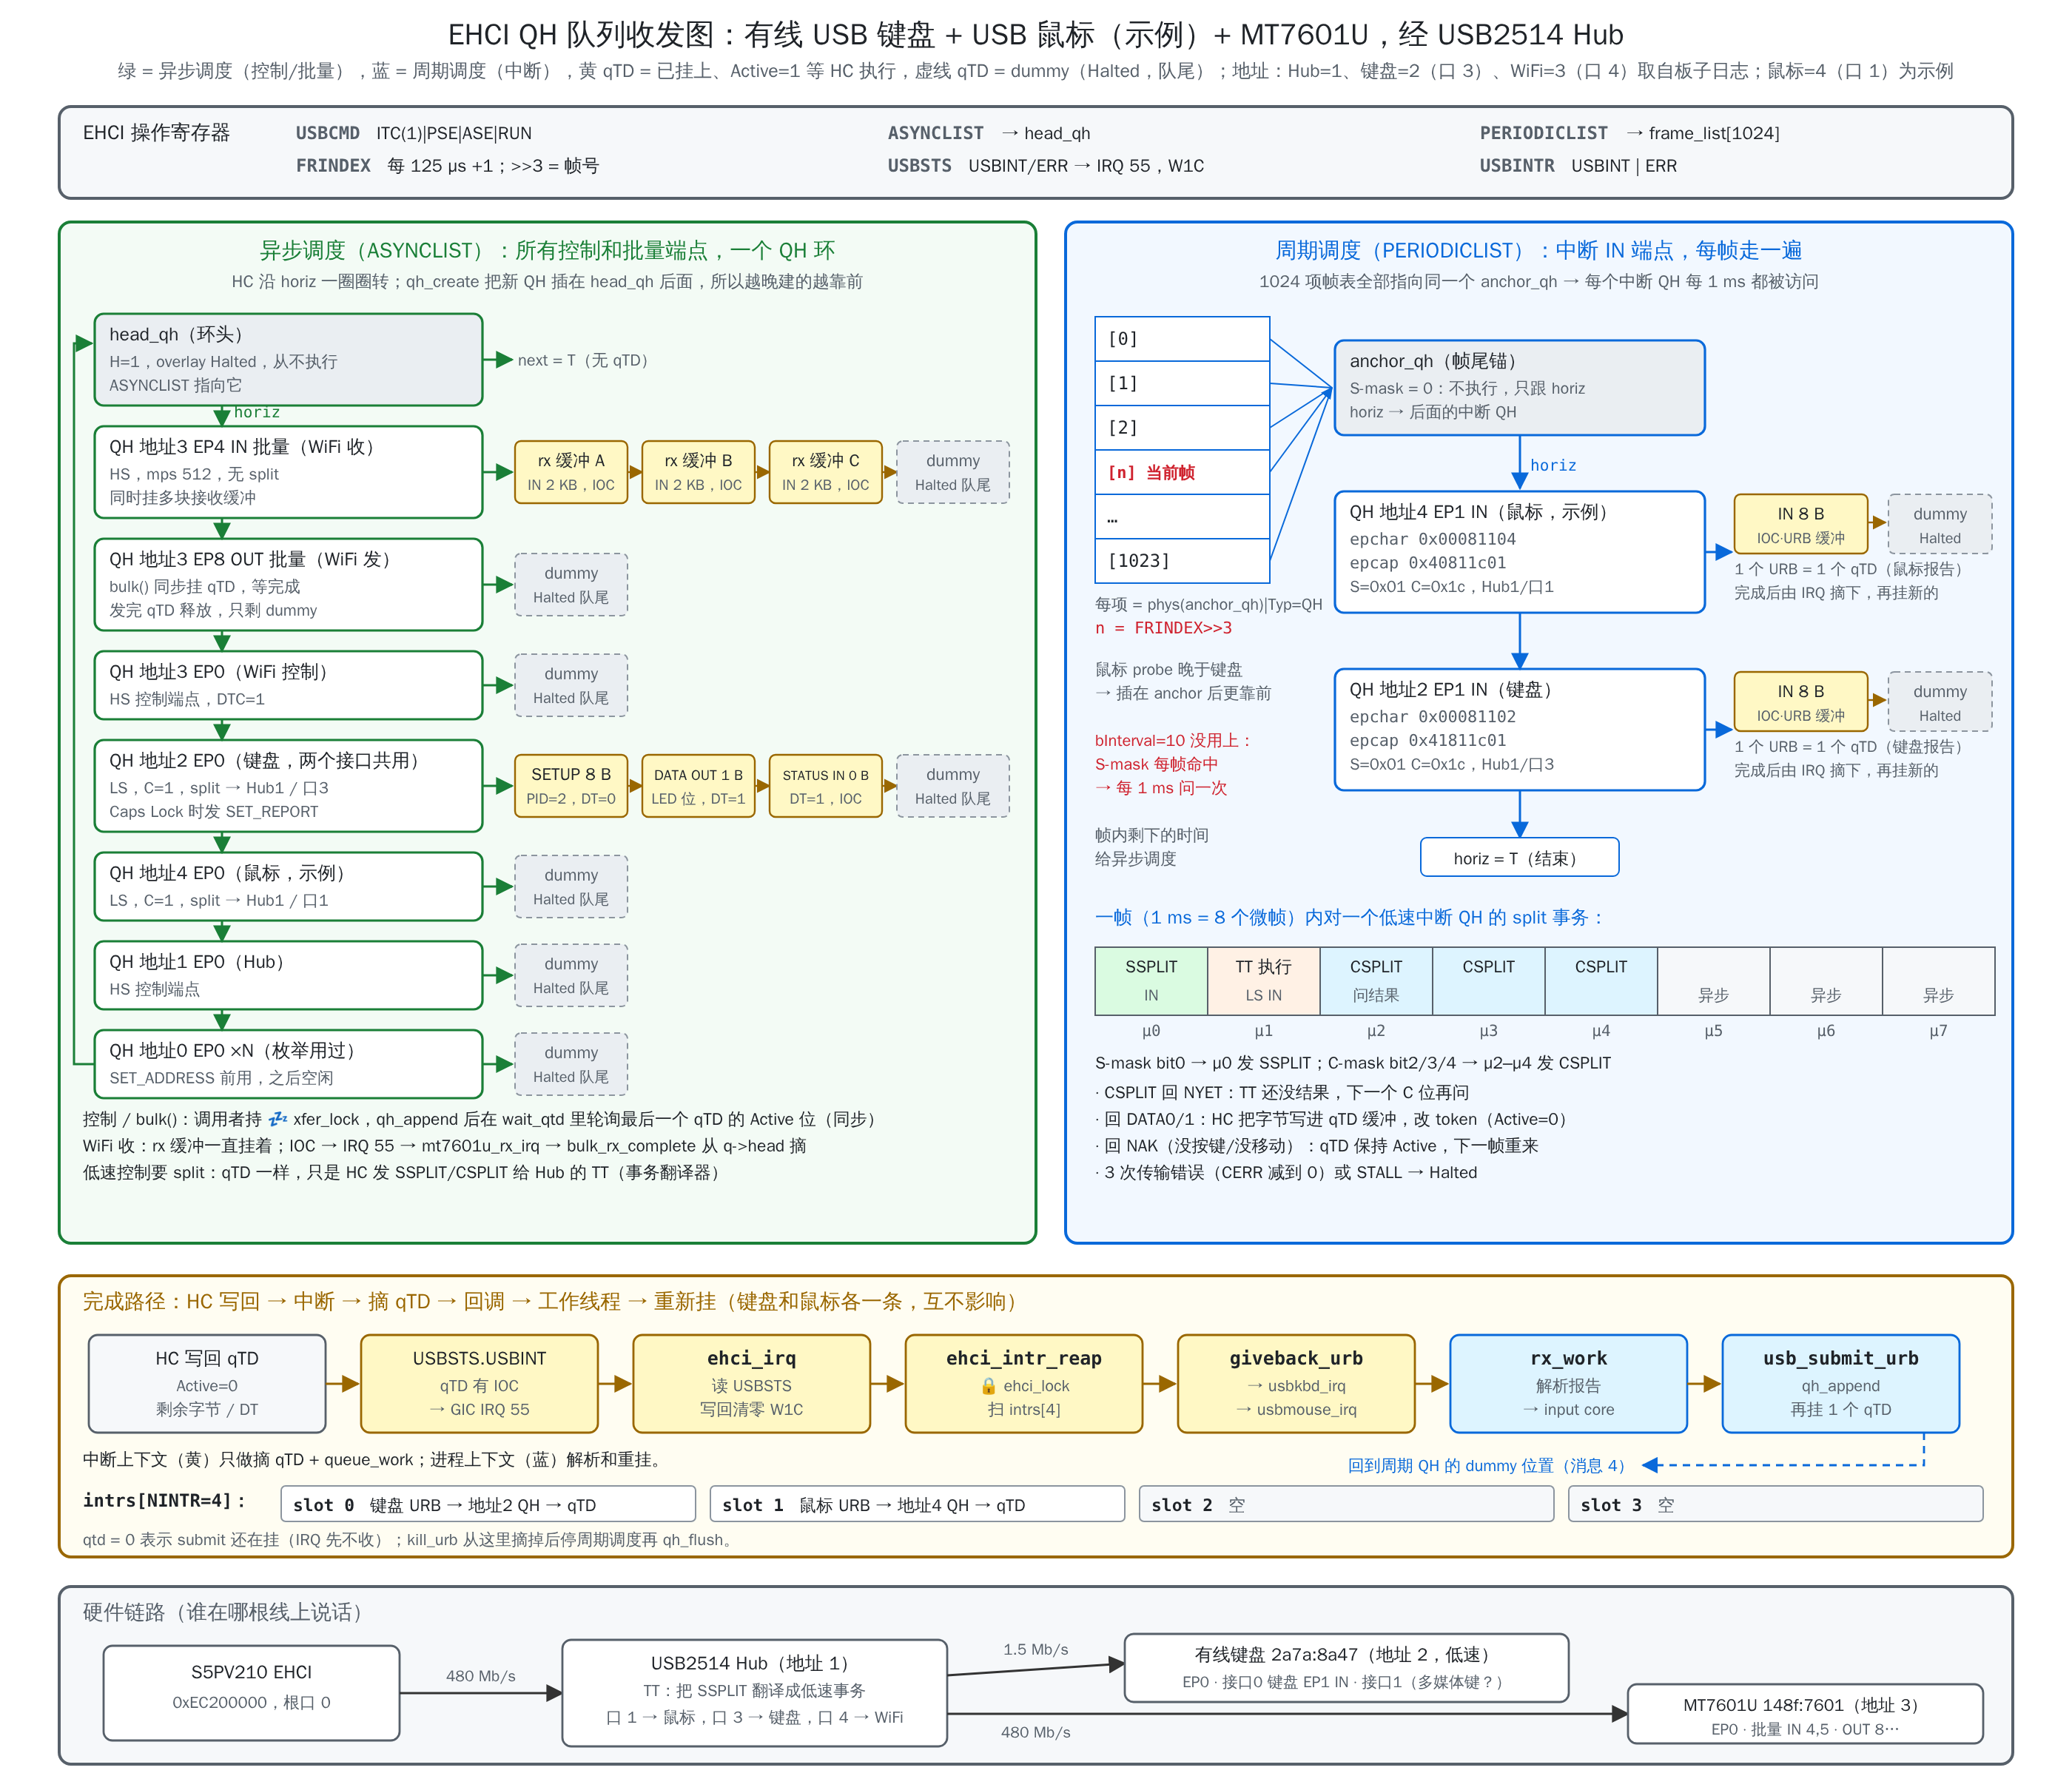
\includegraphics[width=\linewidth]{qh-overview.png}
  \caption{EHCI QH 队列总览：左为异步环（控制、批量），右为周期调度（帧表 → anchor\_qh → 中断 QH）及一帧内的 split 时序，下为完成路径与硬件链路。鼠标为示例。完整图见 \texttt{images/ehci-qh-queues.svg}。}
\end{figure}

\begin{figure}[h]
  \centering
  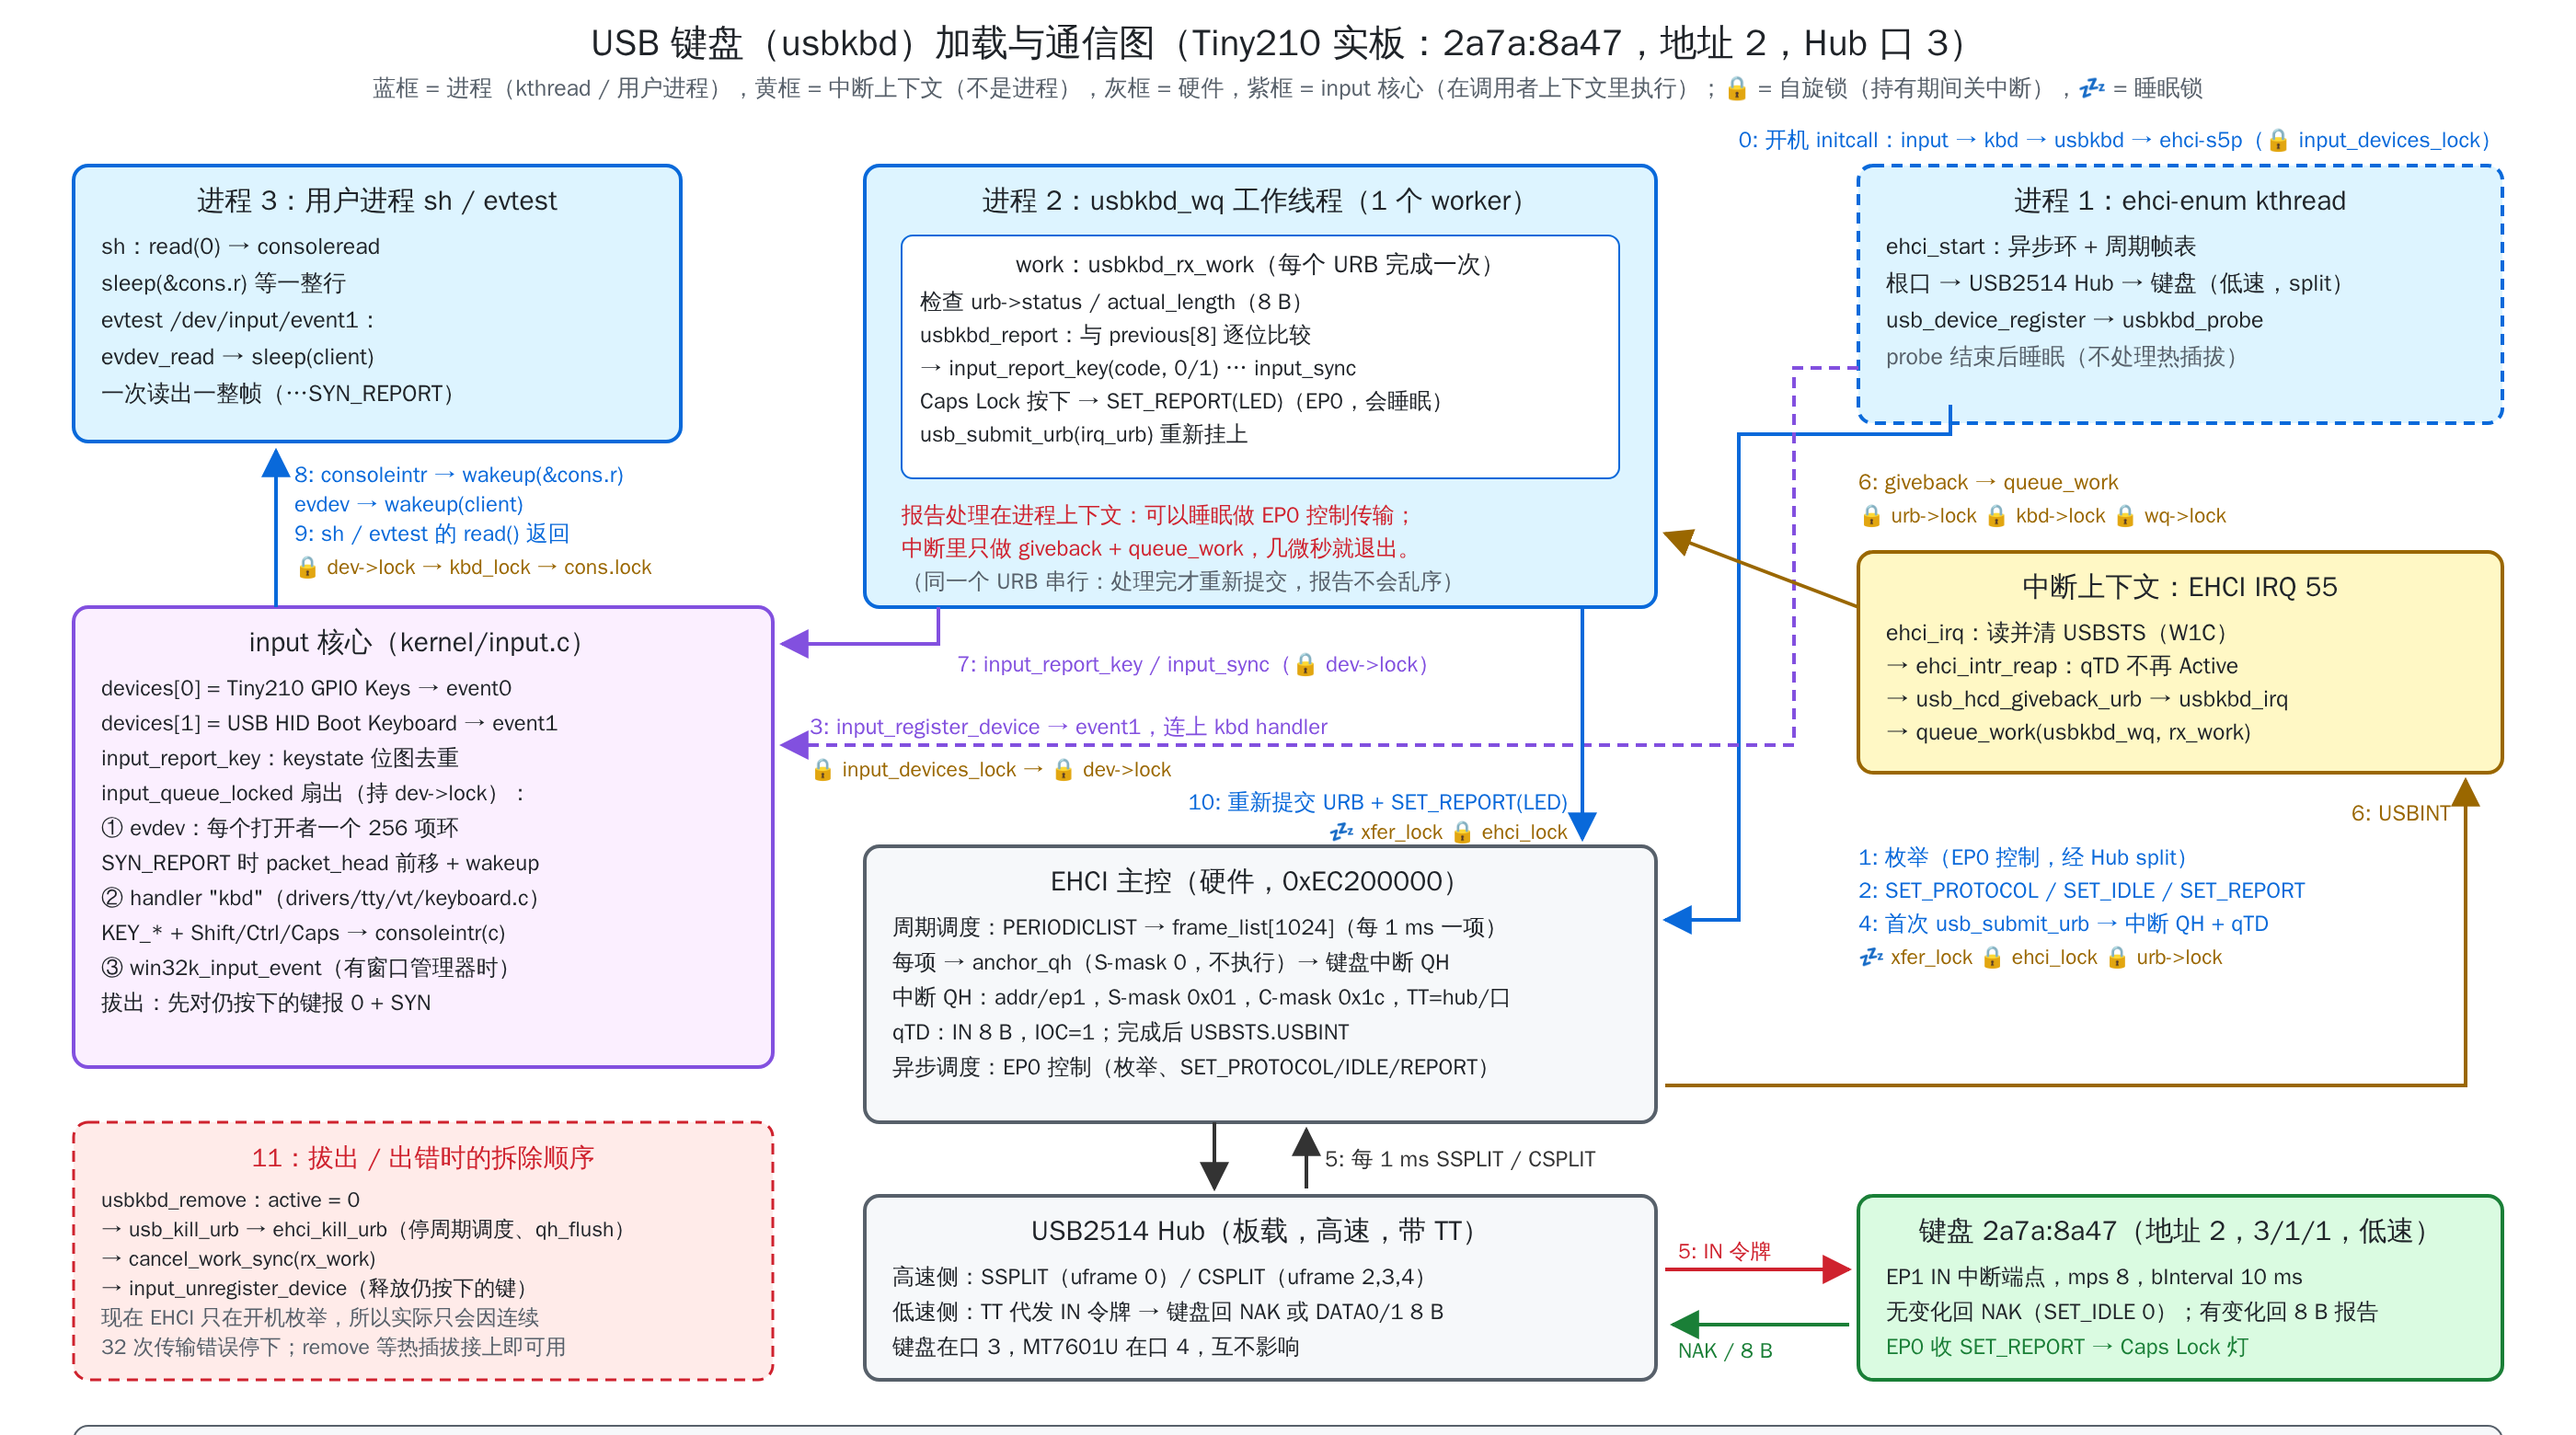
\includegraphics[width=\linewidth]{kbd-overview.png}
  \caption{usbkbd 加载与通信总览（实板：2a7a:8a47，地址 2，Hub 口 3）。完整图见 \texttt{images/usbkbd-comm-steps.svg}。}
\end{figure}

\end{document}
